% $Header: /projects/VU-SAGA/Papers/saga_engine_2006/details.tex,v 1.4 2006/08/13 18:01:00 hkaiser Exp $

The following section will describe certain implementation details
of the SAGA C++ reference implementation. As we will see, our 
implementation gains its flexibility mainly from the combined
application of C++'s compile time and runtime polymorphism features,
i.e. template's and virtual functions respective.

\subsection{General considerations}

  To achieve a maximum of portability, platform independence and code
  reuse, the SAGA C++ reference implementation relies strictly on the
  Standard C++ language features, and uses the C++ Standard and Boost
  libraries wherever possible. 
  
\subsubsection{The SAGA task model}
\label{ssec:tasks}

  A central concept of the SAGA API design is the SAGA task
  model\footnote{\small The motivation for this task model is outside the
  scope of this paper, but is in some detailed described
  in~\cite{saga-paper}.  This paper merely refers to those aspects
  which are relevant to the library design.}.  That model prescribes
  the form of synchronous and asynchronous method calls.  Essentially,
  each method call comes in three variants: as a \I{synchronous call}, 
  as a \I{asynchronous call}, and as a \I{task call}.  The synchronous call is, as
  expected, executed immediately, and has normal return values.  The
  asynchronous and task versions of the calls return a
  \T{saga::task} class instance.  A \T{saga::task} thus represents an asynchronously
  running operation, and has state (\T{Pending, Running, Finished, Failed}).
  Task versions of the method calls return a \T{Pending} task,
  asynchronous versions return a \T{Running} task, i.e. the \T{run()}
  method was called on that task.  For symmetry reason, we added a
  fourth version of method calls, which is again synchronous, but
  returns a \T{Finished} task.
  % i.e. \T{run()} and \T{wait()} have been called.
  The C++ rendering of the SAGA task model is shown in
  figure~\ref{src:tasks}.

\begin{figure}[!ht]
 \begin{center}
  \begin{mycode}[label=SAGA task model]
  {
    using namespace std;
    using namespace saga;

    string src   = "any://host.net//data/src.dat";
    string dest1 = "any://host.net//data/dest1.dat";
    string dest2 = "any://host.net//data/dest2.dat";
    string dest3 = "any://host.net//data/dest3.dat";
    string dest4 = "any://host.net//data/dest4.dat";

    file f (src);

    // normal sync version of the copy method
    f.copy (dest1);

    // the three task versions of the same method
    task t1 = f.copy <task::Sync>  (dest2);
    task t2 = f.copy <task::ASync> (dest3);
    task t3 = f.copy <task::Task>  (dest4);

    // task states of the returned saga::task
    // t1 is in 'Finished' or 'Failed' state
    // t2 is in 'Running'              state
    // t3 is in 'Pending'              state

    t3.run  ();

    t2.wait ();
    t3.wait ();

    // all tasks are 'Finished' or 'Failed' now
  }
  \end{mycode}
  \up
  \up
  \caption{\label{src:tasks}
    The SAGA task model rendered in C++}
 \end{center}
\end{figure}

While we tried to absolutely minimize the use of template's in the 
API layer, we decided to implement the different flavors of the API 
functions with the help of function templates (see figure~\ref{src:tasks}). 
This makes the whole SAGA C++ implementation \I{generic} with respect to 
the synchronicity model, being another reason for providing 
two types of the synchronous function flavors: a direct and a task 
based one.

% \newpage
\subsubsection{The Object Instance Structure}
\label{ssec:pimpl}

As already mentioned, the SAGA API objects are implemented using the PIMPL idiom.
Their only essential member is a \T{boost::smart\_ptr<>} to the 
base class of the implementation object instance\footnote{\small We refer to the 
implementation side of the PIMPL paradigm as \I{impl classes} in this document}, 
keeping it alive. This makes them very 
lightweight and copy able without major overhead, and therefore storable in any 
type of container.

As shown in figure~\ref{fig:object_structure}, any API object instance creates
the corresponding impl instance holding all the instance data
of the SAGA object instance (that are those data which define the state of the 
API object instance, such as the name and current seek position of a file). 
Copying of a API instance therefore shares this state between the copied 
instances, which probably is what a user expects. Moreover, this 
behavior is consistent with anticipated handle based SAGA language bindings 
(such as for C or FORTRAN), where copying the handle representing a SAGA 
object instance naturally means sharing the internal instance data as 
well\footnote{\small A polymorphic \T{saga::object::clone()} method is, however, part 
of the SAGA API, and allows for explicit deep copies of API objects, 
forcing the instance data to be copied as well.}.  

\begin{figure}[!ht]
 \begin{center}
  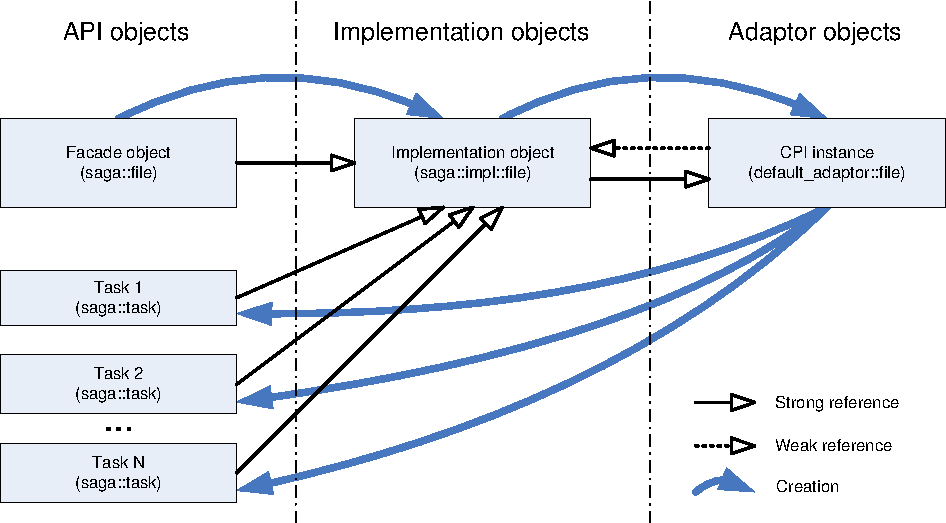
\includegraphics[width=0.47\textwidth]{images/object_structure}
  \caption{\label{fig:object_structure}
    Object instance structure: Copying a API object instance means sharing 
    state, returned tasks keep implementation alive.}
 \end{center}
\end{figure}

Due to the shared
referencing after copies, the impl instances can be kept alive by objects
which depend on their state -- for example, a task keeps the objects
alive for which they represent a asynchronous method call (see
figure~\ref{fig:object_structure}).

The call sequence for creating a SAGA API object instance is shown in
figure~\ref{fig:object_creation}.  Whenever needed, the implementation
creates a CPI object instance implemented in one of the adaptors. The 
adaptor selection, instantiation, and creation of the required CPI object 
instance is implemented generically in the SAGA engine module and is 
used by all API packages. This process is injected into the API packages 
by the macros mentioned before (see section~\ref{ssec:apipackages}).

\begin{figure}[!ht]
 \begin{center}
  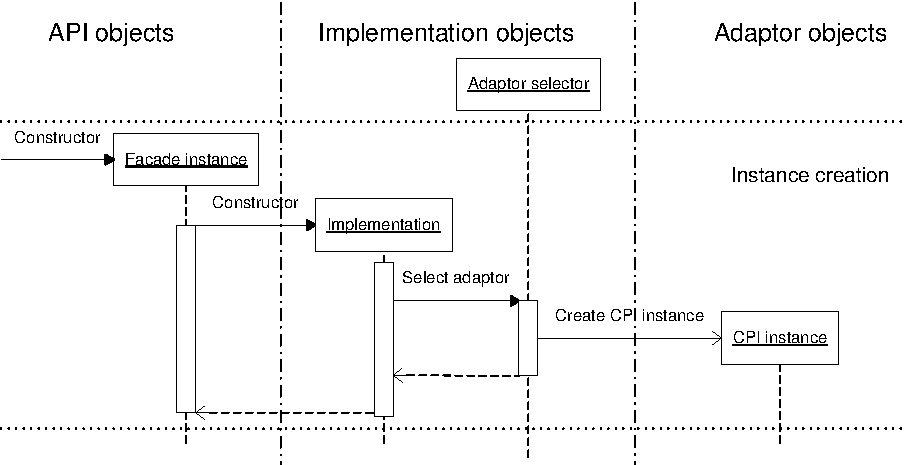
\includegraphics[width=0.47\textwidth]{images/object_lifetime_creation}
  \caption{\label{fig:object_creation}
    Object creation: Sequence diagram depicting the creation of all
    components as showed in figure~\ref{fig:object_structure}. Note, how
    the call is intercepted by a SAGA engine module component to select 
    a appropriate adaptor.}
 \end{center}
\end{figure}

\subsection{Inheritance and PIMPL}

An interesting problem in the strict application of the PIMPL
mechanism lies in the API object hierarchy:  the \T{saga::file} class
for example inherits the \T{saga::ns\_entry} class, which inherits the
\T{saga::object} class.  Additionally, the SAGA specification requires
all these classes to implement additional interfaces.  Now, the PIMPL
paradigm requires all class instances to own exactly \I{one} impl
pointer\footnote{\small{In fact the impl pointer stored in any \T{saga::object}
instance is a \T{boost::smart\_ptr<saga::impl::object>}, i.e. a reference
to the very base class of the implementation object hierarchy.}}, and are 
built using single inheritance only, otherwise we would face object slicing 
problems when copying around the base classes only. To achieve that, 
our implementation does the following:

 \begin{shortlist}
   \item interfaces are added to the most derived classes by duplicating
   			 the interface functions, simplified by the usage of macros 
   			 (interfaces as additional base classes would break the single 
   			 inheritance) \footnote{\small{The usage of macros for this task 
   			 isn't a problem, since, as mentioned above, during the build 
   			 process these get pre-expanded anyways.}},
   \item the impl reference is down-casted and passed to the
   			 constructor of the respective base class.
 \end{shortlist}

For example, the \T{saga::file} construction includes the code
fragments shown in figure~\ref{src:implcon}.

\begin{figure}[!ht]
 \begin{center}
  \begin{mycode}[label=saga::file constructor]
  file::file ([args])
    : ns_entry (new saga::impl::file ([args]))
  { }
  \end{mycode}
  \begin{mycode}[label=saga::ns\_entry constructor, firstnumber=last]
  ns_entry::ns_entry (saga::impl::ns_entry* impl)
    : saga::object (impl)
  { }
  \end{mycode}
  \begin{mycode}[label=saga::object constructor, firstnumber=last]
  object::object (saga::impl::object* impl)
    : impl_ (impl) 
  //  impl_ is a boost::smart_ptr<saga::impl::object>
  { }
  \end{mycode}
  \up
  \up
  \caption{\label{src:implcon}
    Realizing inheritance in PIMPL classes (simplified).  Only the
    \T{saga::object} base class owns an impl pointer.}
 \end{center}
\end{figure}

API classes access the impl pointer through \T{get\_impl()}, which, in
derived classes, implies a static up-cast for the base class' impl
pointer.  As an example, the implementation of \T{get\_impl()} for the
\T{saga::ns\_entry} class is shown in figure~\ref{src:getimpl}.  

\begin{figure}[!ht]
 \begin{center}
  \begin{mycode}[label=saga::ns\_entry.get\_impl() ]
  boost::shared_ptr <saga::impl::ns_entry> 
         ns_entry::get_impl (void) const
  { 
    // base class is saga::object
    return (boost::shared_ptr <saga::impl::ns_entry> 
              (this->saga::object::get_impl (), 
               boost::detail::static_cast_tag ()
           )  );
  }
  \end{mycode}
  \up
  \up
  \caption{\label{src:getimpl}
    \T{get\_impl()} implies a static cast of the base class impl
    pointer.}
 \end{center}
\end{figure}

The implementation objects resemble the structure of the API objects.
These are derived from a common base class as well and contain, somewhere 
in their own hierarchy, similar objects as the API objects. 
The \T{saga::impl::file} class\footnote{\small{The \T{saga::impl::file} 
class for example is the implementation equivalent to the \T{saga::file} class, as 
we kept all API classes in \T{namespace~saga} and all corresponding 
implementation classes in \T{namespace~saga::impl}.}} inherits the 
\T{saga::impl::ns\_entry} class, which inherits the implementation 
specific \T{saga::impl::proxy} class, which is derived from the common 
\T{saga::impl::object} class.  Thus, the
class hierarchy on the implementation side of the PIMPL paradigm
reflects the API side of the class hierarchy, which ensures
the correct casting behavior in the \T{get\_impl()} respective methods.


\subsection{State Management}

Section~\ref{ssec:pimpl} made some remarks about object state, in relation to
state sharing of objects after shallow copies.  We want to describe the object
state management of our SAGA implementation in some more detail, as state
management is a central element on several layers.  The mentioned state
management in the PIMPL layers allows, as we have seen, to share state between
separate API object instances.   On a different layer, the adaptors represent
operations on these object instances, and need to maintain state as well.
Complicating on adaptor level is the fact that the object state can (and in
general will) be changed by several adaptors (remember: adaptors are selected
at runtime, and may change for each API function invocation).  For state 
management, we hence distinguish between three types of instance data.

\begin{shortlist}
	\item \I{Instance data} represent the state of API objects (e.g. file name, 
			file pointer etc.). These are predefined and not amendable by the adaptor
			since they mainly represent common data either passed from the constructor,
			or needed for consistent state management on API level.
	\item \I{Adaptor data} represent the state of CPI objects (e.g. open connections, 
			remote handles etc.) and are shared between all instances of all different 
			CPI object types\footnote{\small{For instance such as file and directory 
			CPI implementations commonly implemented by one adaptor.}} implemented by 
			a single adaptor and corresponding to a single adaptor instance. These are 
			naturally implemented by the adaptor writer as member data of the corresponding 
			adaptor type.
	\item \I{Adaptor-instance data} represent the state shared between all CPI 
			instances created for a single API object and implemented by the same 
			adaptor. The most natural way were to implement this type of instance 
			data as members of the corresponding CPI object. Unfortunately this is 
			not possible since we cannot guarantee, that the very same CPI \I{instance}
			will get reused for different API function calls on a particular API object 
			instance. For this reason the adaptor-instance data is stored in a
			map in the impl object, identified by a universal unique identifier (UUID)
			\footnote{\small{All object instances in our SAGA implementation have 
			an associated UUID allowing them to be uniquely identified.}}.
\end{shortlist}

The lifetime of any type of the instance data is maintained by the SAGA engine 
module, which significantly simplifies writing of adaptors.

All three types of instance data have to be carefully protected from race 
conditions possibly caused by the multithreaded nature of the overall implementation.
Every adaptor needs to access at least one type of these instance data. 
So our implementation provides helper classes allowing to simplify the 
correct locking of the instance data. Please refer to figure~\ref{src:instancedata} 
to get an example, how to use these predefined wrappers for accessing the instance 
data members of a \T{saga::file} object. The main trick is,
that the wrapper classes implement a \T{operator->()} returning a pointer
to the locked instance data. This lock is aquired during construction
and is released during destruction of the wrapper instance.

Additionally, uniform state management is very important to allow for
object state persistency in the future, with minimal impact on the existing
code base.

\begin{figure}[!ht]
 \begin{center}
  \begin{mycode}[label=Instance data type declaration]
    // file_instance_data can be used for the
    // thread safe access to instance data
    using namespace saga::adaptors;
    typedef instance_data <file_cpi_instance_data> 
        file_instance_data;
  \end{mycode}
  \begin{mycode}[label=Instance data usage, firstnumber=last]
     void file_cpi_impl::sync_read ([args])
     {
       // ... calculate 'bytes_read'
       { 
         // the constructor aquires a lock
         file_instance_data data (this);

         // adjust instance data member 'pointer_'
         // (seek position) with number of bytes read
         data->pointer_ += bytes_read;

       } // lock goes out of scope here
     }
  \end{mycode}
  \up
  \up
  \caption{\label{src:instancedata}
    Definition and use of a wrapper class to access instance 
    data in a thread safe manner.}
 \end{center}
\end{figure}


\subsection{Generic Call Routing}
\label{ssec:routing}

A couple of times we referred to the engines ability to generically
route SAGA API method calls to adaptors.  The essential idea of that
routing mechanism is to represent these calls as abstract objects, and
to redirect their execution depending on several attributes, and
depending on the availability of suitable adaptors.  For example,
a asynchronous method call for a |saga::file| instance is preferably
directed to a asynchronous file adaptor, or, if such is not available,
to a synchronous file adaptor (the method gets executed in a thread
than, making it asynchronous to some extend), or, if that is not
available either, returns an error (NotImplemented).

\newpage
That routing mechanism allows for 
\begin{shortlist}
   \item trivial (synchronous) adaptor implementations, 
   \item late binding: a different adaptor can be selected
         for each call, even on the same API object instance, 
   \item the application of various adaptor selection strategies, e.g. 
         based on adaptor meta data, user preferences and heuristics, 
   \item latency hiding, e.g. by clustering related method calls (bulk
         optimization, see section~\ref{ssec:bulks}), or by 
         automatic load distribution over multiple adaptors (not 
         implemented yet).
\end{shortlist}

Figure~\ref{fig:object_functioncall} depicts the point in the sequence of calls
where this call routing mechanism is injected by the SAGA engine.

\begin{figure}[!ht]
 \begin{center}
  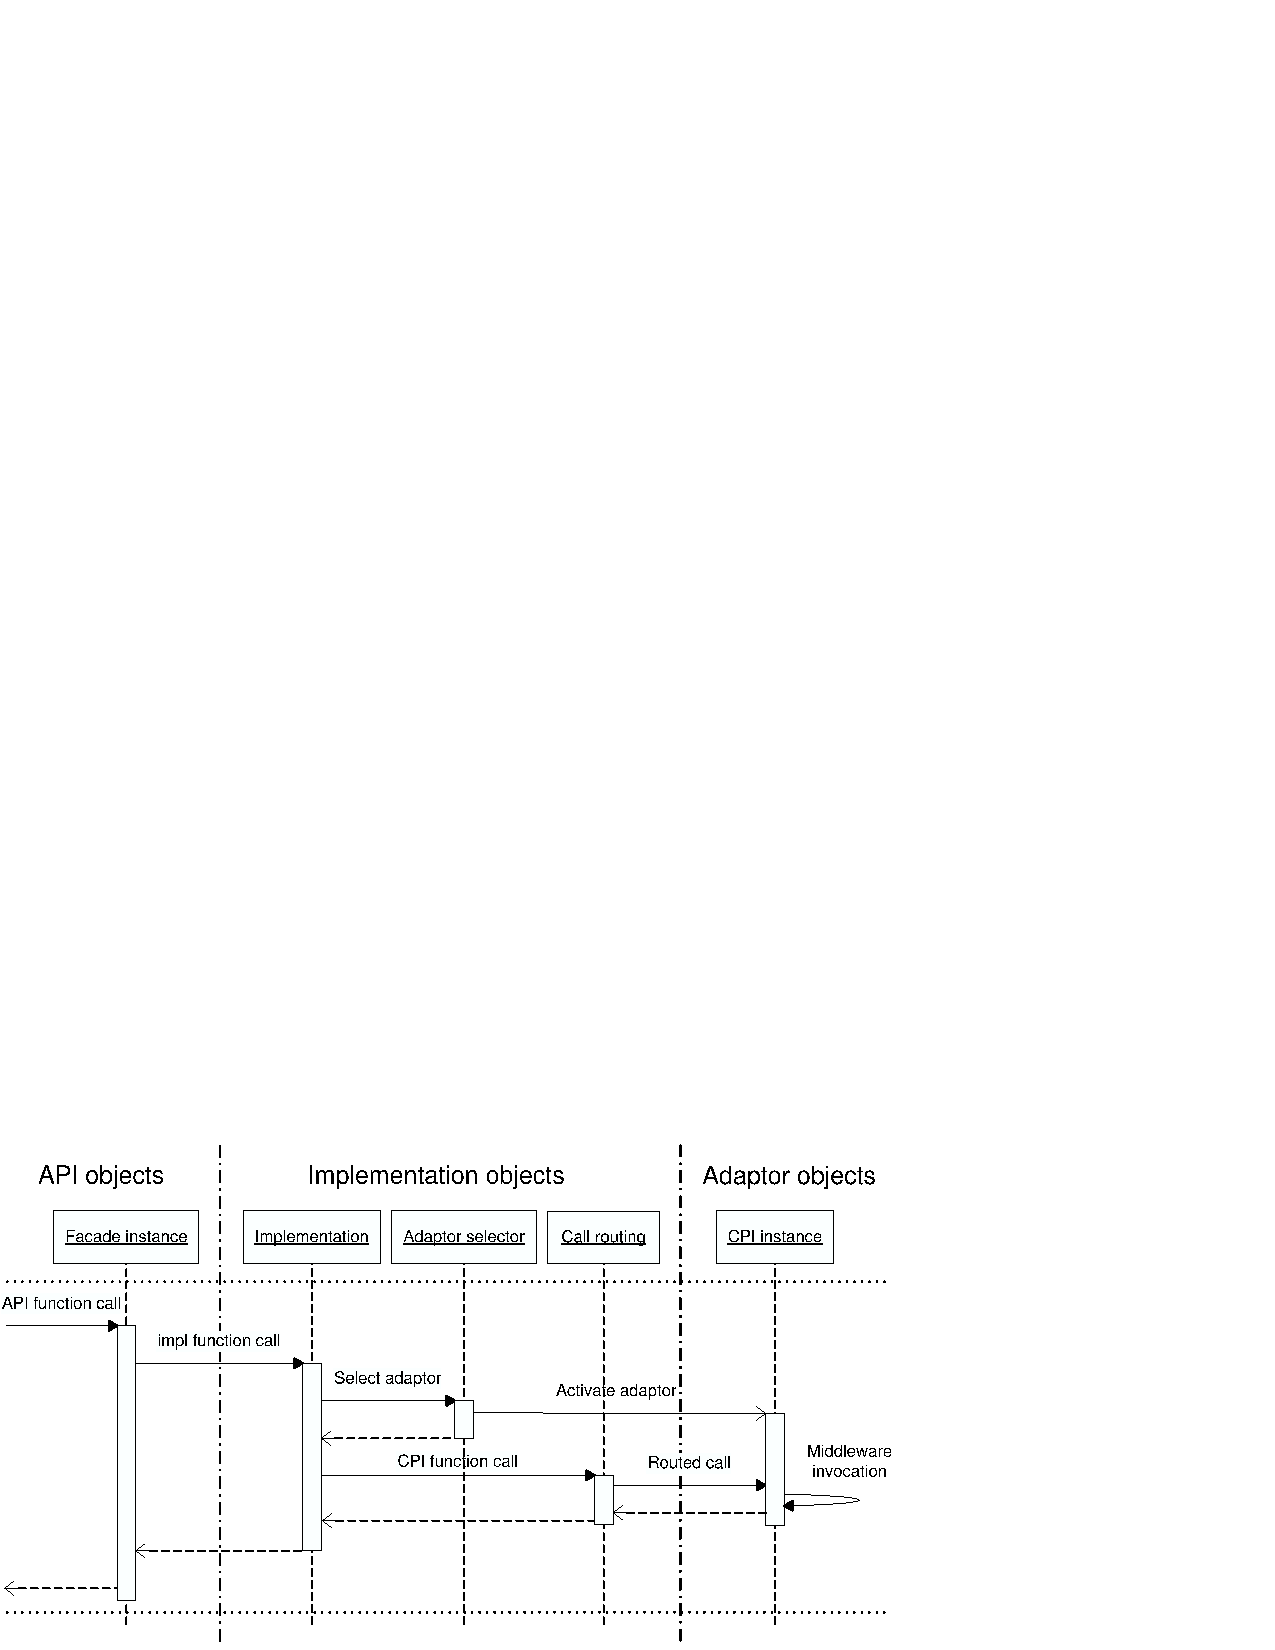
\includegraphics[width=0.47\textwidth]{images/object_lifetime_functioncall}
  \caption{\label{fig:object_functioncall}
    API function call: Diagram illustrating the execution sequence through 
    the different object instances during a call to any adaptor supplied 
    function.}
 \end{center}
\end{figure}

\subsubsection{Sync/Async Routing}

As the SAGA API methods come in synchronous and asynchronous flavors
(see section~\ref{ssec:tasks}), adaptors would normally need to implement
the methods in these two flavors as well.  That, however, has been
avoided by providing fallback implementations in the
SAGA engine, if needed.   The synchronous behavior is very easy 
to model: the asynchronous implementation has to be executed and to be waited
for.  The asynchronous behavior however requires the synchronous
implementation to be wrapped into a thread.  That thread then
represents the asynchronous remote operation -- internally, that
thread is represented as a |saga::impl::task| instance.
The realization of the |saga::impl::task| class bases on a
implementation of the \I{futures} paradigm, a concurrency abstraction 
first proposed for MultiLisp~\cite{futures}.  

It must be noted that this mechanism has a number of drawbacks:  (a)
the operation is not really asynchronous, as for example a dropped
connection will likely cause it to fail; (b) the CPI instance
executing the method still blocks (it is synchronous), which can, if
badly implemented, cause locks on shared data structures; (c) the SAGA
task model is, at some point in the future, to be extended, and tasks
are then supposed to be able to survive an application life time --
that would break the current implementation.

However, the mechanism allows simplifying adaptor implementations
greatly, as most of the current existing grid middleware is \I{not}
fully asynchronous anyway.



\subsubsection{Bulk optimizations}
\label{ssec:bulks}

Bulk optimizations represent a special form of latency hiding:
multiple related, independent method invocations are clustered into a
single call.  That reduces the amount of remote communication needed
to execute that method.  A very common example is the execution of
multiple remote I/O operations, which can be clustered in a single
operation (the POSIX scattered I/O, |readv/writev (2)|, have a similar
objective).  Our implementation allows to cluster tasks which are
collectively run in a task container (see
figure~\ref{src:taskcontainer} for an example) to be clustered according to the
method signature (e.g. same methods on the same object instance form
one bulk), and can then passed to adaptors which implement bulk
versions of that method.  If that bulk version is nowhere implemented,
the methods are called one-by-one, as would be the default.


\begin{figure}[!ht]
 \begin{center}
  \begin{mycode}[label=Usage of SAGA task\_container]
  {
    using namespace std;
    using namespace saga;
    using namespace boost::assign;

    string src ("any://host.net//data/src.dat");
    file   f   (src);

    vector <string> dest;
    dest += "any://host.net//data/dest1.dat",
            "any://host.net//data/dest2.dat",
            "any://host.net//data/dest3.dat",
            "any://host.net//data/dest4.dat";

    // create a saga::task_container
    task_container tc;

    vector<string>::iterator end = dest.end ();
    for (vector<string>::iterator it = dest.begin (); 
         it != end; ++it)
    {
      // add 'Pending' tasks to the task_container
      tc.add (f.copy <task::Task> (*it));
    }
    
    // run all tasks, then wait for all
    // bulk optimization is applied here.
    tc.run  ();
    tc.wait ();

    // all tasks are 'Finished' or 'Failed' now
  }
  \end{mycode}
  \up
  \up
  \caption{\label{src:taskcontainer}
    Usage of the SAGA \T{task\_container} class: This example 
    illustrates, how the SAGA C++ implementation provides a 
    simple and natural way to integrate grid related remote
    operations with well known C++ paradigms.}
 \end{center}
\end{figure}

% \newpage

\subsection{Adaptor Selection}

The selection of suitable adaptors at runtime represents is a central
component in the represented library implementation (see
figure~\ref{fig:object_functioncall}).  It is, in general, a very simple
mechanism: on loading, the adaptor components register their
\I{capabilities} in the adaptor registry.  If a method is to be
executed, the adaptor selector searches that registry for all adaptors
which implement that methods capability.  All suitable adaptors are
then ordered (best/most suitable first), and are tried one-by-one,
until the method invocation succeeds. The adaptor selection again is 
routed through SAGA engine components, generically implementing this for 
any function to be routed to a CPI instance.

Now, that simple mechanism has a number of potential pitfalls.  For
one, as can be seen in figure~\ref{fig:object_creation}, a number of
adaptor instances (i.e. CPI instances) must be created.  That can
imply remote operations, and hence significant latency.  Secondly, the
ordering of adaptors is very difficult, as it is hard to specify what
constitutes a \I{good} or \I{suitable} adaptor.  One metric is of
course the availability of the required capability.  Another utilized
metric is the preference of adaptors providing the correct flavor
(synchronous/asynchronous implementation).  More elaborate metrics
however will strongly depend on the implementation.

Our library however allows adaptors to specify additional, key/value
based meta data, and also allows to exchange the adaptor selection
component.  That way it is possible to (a) add additional meta data to
adaptors (e.g. '|secure=yes/no|', or |'type=local/remote'|), and (b)
add selection mechanism which evaluate and honor these meta data.

We apply a very simple optimization to the described scheme: if an
adaptor was successfully invoked for an objects method call, the same
adaptor is tried first on the next method call on the same object.
That way, the adaptor selection is performed only once (on creation
creation), and only repeated if any method invocation fails.


\subsection{Utilization of Macros}
\label{ssec:macros}

Our SAGA implementation makes extensive use of C++ preprocessor
macros.  That fact might be perceived as a design flaw, at least by
some readers, and we have been very hesitant to utilize macros as
extensively as we do ourselfes.  However, the benefits for the end user
and other programmers(!) seem currently to outweigh the problems we are
introducing, such as limited debugging abilities\footnote{\small As
mentioned in section~\ref{ssec:apipackages}, we are using Boost.Wave
features to pre-generate partially macro expanded sources to overcome 
the disadvantages of plain macros, hence simplifying debugging and 
improving readability.}.

We use macros in three different functions: for defining the API, for
implementing API level interfaces, and for implementing the API on the
implementation side of the PIMPL layer.

Figure~\ref{src:sidl} shows a part of the SAGA API definition in
Scientific IDL (SIDL, \cite{sidl}).  The second part of the same
figure shows the representation of the same SIDL segment in our
implementation: the class depicted there is essentially complete!  Adding
a new API package can be done in minutes, and, in fact, is easy to
automate (see section~\ref{ssec:apipackages}).  The macros expand to all
required flavors of the API (synchronous, asynchronous, task based, and 
task based synchronous -- see
section~\ref{ssec:tasks}).  The implementation macros retrieve the impl
pointer via |get_impl()| (see sec~\ref{ssec:pimpl}), and invoke the
respective impl method.  

\begin{figure}[!ht]
 \begin{center}
  \begin{mycode}[label=saga::file in SIDL]
  class file : extends         saga::ns_entry,
               implements-all  saga::monitorable
  {
    // ctor and dtor removed in this example
    is_file     (in  int            flags = None,
                 out bool           test);
    read        (inout array<byte>  buffer,
                 in    int          len_in,
                 out   int          len_out);
  // ...
  }
  \end{mycode}
  \begin{mycode}[label=saga::file in C++ Macros, firstnumber=last]
  // file.hpp
  class file 
    : public saga::ns_entry
  {
    protected:
      boost::shared_ptr <impl::file> get_impl () const;

    private:
      PRIV_0      (bool,    is_file, int);
      PRIV_2      (ssize_t, read,    char*, size_t);
  // ...

    public:
      PUB_1_DEF_1 (bool,    is_file, int,   None);
      PUB_2_DEF_0 (ssize_t, read,    char*, size_t);
  // ...
  }

  // file.cpp
  IMP_2 (file, ssize_t, read, char*, size_t);
  \end{mycode}
  \begin{mycode}[label=saga::impl::file in C++ Macros, firstnumber=last]
  // impl/file.hpp
  class file 
    : public saga::impl::ns_entry
  {
    public:
      IMP_DECL_1 (bool   , is_file, int);
      IMP_DECL_2 (ssize_t, read,    char*, size_t);
  // ...
  }
  
  // impl/file.cpp
  IMP_IMPL_1 (file, file_cpi, bool, is_file, int);
  IMP_IMPL_2 (file, file_cpi, ssize_t, read, char*, 
              size_t);
  \end{mycode}
  \up
  \up
  \caption{\label{src:sidl}
    Macro base API definition and implementation (macro names 
    abbreviated)}
 \end{center}
\end{figure}


On the implementation side, the API is again specified and implemented
by macros -- these macros expand to implementations which invoke the
generic call routing described in section~\ref{ssec:routing}.  That way,
the impl classes are similarly thin and lightweight as the API
itself.  The examples in figure~\ref{src:sidl} do not show that the
definition of the CPI are done by similar macros -- these macros
define an abstract base class, which is then implemented by the
adaptors, essentially implementing the original SAGA API, and
providing the required grid capabilities.

Our implementation uses macros in well defined locations, and they
allow for simple extensibility of the API.  In fact, we consider the
usage of our SAGA implementation to implement other APIs for
distributed systems, and also to re-implement earlier grid APIs for
backward compatibility -- the macros as shown, and the generic call
routing, make that a very simple exercise.

